% Plain ICLR-style MIRAGE pipeline (black/white, Times). Compile with pdflatex; include with
% 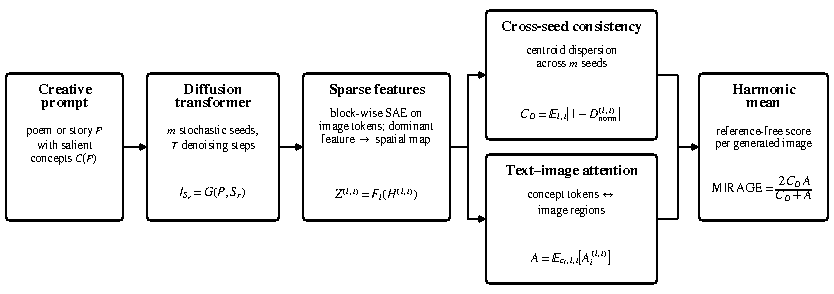
\includegraphics[width=\linewidth]{mirage_pipeline_plain.pdf}.  NOT compiled in the authoring
% environment (no LaTeX there) -- the matching, rendered version is mirage_pipeline_plain.pdf.
\documentclass[tikz,border=3pt]{standalone}
\usepackage[T1]{fontenc}
\usepackage{mathptmx}
\usepackage{amsmath,amssymb}
\usetikzlibrary{arrows.meta,calc}

\tikzset{
  stage/.style={draw=black,rounded corners=2pt,line width=.5pt,fill=white,align=center,
                inner sep=3pt,font=\scriptsize},
  arr/.style={-{Stealth[length=3pt,width=2.6pt]},line width=.5pt},
}
\newcommand{\ttl}[1]{{\footnotesize\bfseries #1}\\[2pt]}

\hyphenpenalty=10000\exhyphenpenalty=10000
\begin{document}
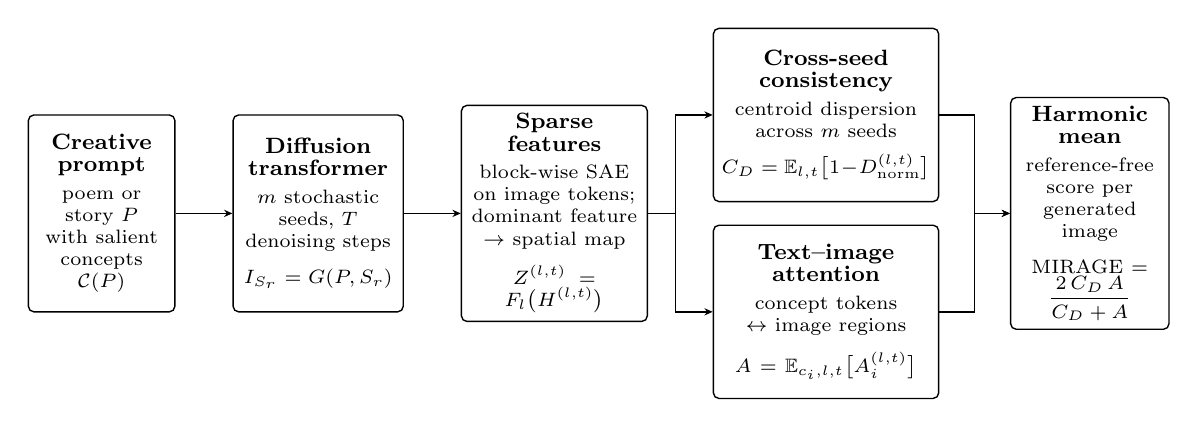
\begin{tikzpicture}
  % column centres (cm); single boxes on y=0, the two signals stacked at y=+-1.25
  \node[stage,text width=1.65cm,minimum height=2.5cm] (s1) at (0,0)
    {\ttl{Creative prompt}poem or story $P$ with salient concepts $\mathcal{C}(P)$};
  \node[stage,text width=1.95cm,minimum height=2.5cm] (s2) at (2.75,0)
    {\ttl{Diffusion transformer}$m$ stochastic seeds, $T$ denoising steps\\[5pt]$I_{S_r}=G(P,S_r)$};
  \node[stage,text width=2.15cm,minimum height=2.5cm] (s3) at (5.75,0)
    {\ttl{Sparse features}block-wise SAE on image tokens; dominant feature $\to$ spatial map\\[5pt]$Z^{(l,t)}=F_l\big(H^{(l,t)}\big)$};
  \node[stage,text width=2.65cm,minimum height=2.2cm] (s4) at (9.2,1.25)
    {\ttl{Cross-seed consistency}centroid dispersion across $m$ seeds\\[5pt]$C_D=\mathbb{E}_{l,t}\big[1-D^{(l,t)}_{\mathrm{norm}}\big]$};
  \node[stage,text width=2.65cm,minimum height=2.2cm] (s5) at (9.2,-1.25)
    {\ttl{Text--image attention}concept tokens $\leftrightarrow$ image regions\\[5pt]$A=\mathbb{E}_{c_i,l,t}\big[A_i^{(l,t)}\big]$};
  \node[stage,text width=1.8cm,minimum height=2.5cm] (s6) at (12.55,0)
    {\ttl{Harmonic mean}reference-free score per generated image\\[5pt]$\mathrm{MIRAGE}=\dfrac{2\,C_D\,A}{C_D+A}$};

  % arrows (orthogonal fork and merge)
  \draw[arr] (s1.east)--(s2.west);
  \draw[arr] (s2.east)--(s3.west);
  \draw[arr] (s3.east)--++(.35,0) |- (s4.west);
  \draw[arr] (s3.east)--++(.35,0) |- (s5.west);
  \draw[arr] (s4.east)--++(.45,0) |- (s6.west);
  \draw[arr] (s5.east)--++(.45,0) |- (s6.west);
\end{tikzpicture}
\end{document}
